\chapter{Конструкторский раздел}
\label{cha:design}

\section{Общая архитектура приложения}
В состав программного обеспечения входит только загружаемый модуль ядра, следящий за вызовом нужных функций, с поледующией отправкой информации о них клиенту напрямую из пространства ядра.

\section{Перехват функций}

Каждую перехватываемую функцию можно описать следующей структурой:
\begin{lstlisting}[language=c++,,escapeinside={(@}{@)},caption={ftrace\_hook}]
/**
* struct ftrace_hook - описывает перехватываемую функцию
*
* @name:       имя перехватываемой функции
*
* @function:   адрес функции-обёртки, которая будет вызываться вместо
*              перехваченной функции
*
* @original:   указатель на место, куда следует записать адрес
*              перехватываемой функции, заполняется при установке
*
* @address:    адрес перехватываемой функции, выясняется при установке
*
* @ops:        служебная информация ftrace, инициализируется нулями,
*              при установке перехвата будет доинициализирована
*/
struct ftrace_hook {
	const char *name;
	void *function;
	void *original;

	unsigned long address;
	struct ftrace_ops ops;
};
\end{lstlisting}

Пользователю необходимо заполнить только первые три поля: name, function, original. Остальные поля считаются деталью реализации. Описание всех перехватываемых функций можно собрать в массив и использовать макросы, чтобы повысить компактность кода:

\newpage
\begin{lstlisting}[language=c++,,escapeinside={(@}{@)},caption={ftrace\_hook define}]
#define HOOK(_name, _function, _original)       \
		{                                       \
			.name = (_name),                    \
			.function = (_function),            \
			.original = (_original),            \
		}

static struct ftrace_hook hooked_functions[] = {
	HOOK("sys_clone",   fh_sys_clone,   &real_sys_clone),
};
\end{lstlisting}

Сигнатуры функций должны совпадать один к одному. Без этого, очевидно, аргументы будут переданы неправильно и всё пойдёт под откос. Для перехвата системных вызовов это важно в меньшей степени, так как их обработчики очень стабильные и для эффективности аргументы принимают в том же порядке, что и сами системные вызовы.

\subsection{Инициализация ftrace}
Для начала нам потребуется найти и сохранить адрес функции, которую мы будем перехватывать. Ftrace позволяет трассировать функции по имени, но нам всё равно надо знать адрес оригинальной функции, чтобы вызывать её.

Добыть адрес можно с помощью kallsyms — списка всех символов в ядре. В этот список входят все символы, не только экспортируемые для модулей. Получение адреса перехватываемой функции выглядит примерно так:
\begin{lstlisting}[language=c++,,escapeinside={(@}{@)},caption={resolve\_hook\_address}]
static int resolve_hook_address(struct ftrace_hook *hook)
{
	hook->address = kallsyms_lookup_name(hook->name);

	if (!hook->address) {
		pr_debug("unresolved symbol: %s\n", hook->name);
		return -ENOENT;
	}

	*((unsigned long*) hook->original) = hook->address;

	return 0;
}
\end{lstlisting}

Дальше необходимо инициализировать структуру ftrace\_ops. В ней обязательным полем является лишь func, указывающая на коллбек, но нам также необходимо установить некоторые важные флаги:
\begin{lstlisting}[language=c++,,escapeinside={(@}{@)},caption={fh\_install\_hook}]
int fh_install_hook(struct ftrace_hook *hook)
{
	int err;
	
	err = resolve_hook_address(hook);
	if (err)
		return err;
	
	hook->ops.func = fh_ftrace_thunk;
	hook->ops.flags = FTRACE_OPS_FL_SAVE_REGS | FTRACE_OPS_FL_IPMODIFY;
	
	err = ftrace_set_filter_ip(&hook->ops, hook->address, 0, 0);
	if (err) {
		pr_debug("ftrace_set_filter_ip() failed: %d\n", err);
		return err;
	}
	
	err = register_ftrace_function(&hook->ops);
	if (err) {
		pr_debug("register_ftrace_function() failed: %d\n", err);
		ftrace_set_filter_ip(&hook->ops, hook->address, 1, 0);
		return err;
	}
	
	return 0;
}
\end{lstlisting}

\newpage
Выключается перехват аналогично, только в обратном порядке:
\begin{lstlisting}[language=c++,,escapeinside={(@}{@)},caption={fh\_remove\_hook}]
void fh_remove_hook(struct ftrace_hook *hook)
{
	int err;
	
	err = unregister_ftrace_function(&hook->ops);
	if (err) {
		pr_debug("unregister_ftrace_function() failed: %d\n", err);
	}
	
	err = ftrace_set_filter_ip(&hook->ops, hook->address, 1, 0);
	if (err) {
		pr_debug("ftrace_set_filter_ip() failed: %d\n", err);
	}
}
\end{lstlisting}

После завершения вызова unregister\_ftrace\_function() гарантируется отсутствие активаций установленного коллбека в системе (а вместе с ним — и наших обёрток). Поэтому мы можем, например, спокойно выгрузить модуль-перехватчик, не опасаясь, что где-то в системе ещё выполняются наши функции.

\subsection{Выполнение перехвата функций}

Ftrace позволяет изменять состояние регистров после выхода из коллбека. Изменяя регистр \%rip — указатель на следующую исполняемую инструкцию,— мы изменяем инструкции, которые исполняет процессор — то есть можем заставить его выполнить безусловный переход из текущей функции в нашу. Таким образом мы перехватываем управление на себя.

Коллбек для ftrace выглядит следующим образом:
\begin{lstlisting}[language=c++,,escapeinside={(@}{@)},caption={fh\_remove\_hook}]
static void notrace fh_ftrace_thunk(unsigned long ip, 
	unsigned long parent_ip, struct ftrace_ops *ops, 
	struct pt_regs *regs)
{
	struct ftrace_hook *hook = container_of(ops, struct ftrace_hook, ops);
	regs->ip = (unsigned long) hook->function;
}
\end{lstlisting}

Функция-обёртка, которая вызывается позже, будет выполняться в том же контексте, что и оригинальная функция. Поэтому там можно делать то же, что позволено делать в перехватываемой функции. Например, если перехватывается обработчик прерывания, то спать в обёртке нельзя.

\subsection{Схема работы перехвата}

Рассмотрим пример: терминале набирается команда ls, чтобы увидеть список файлов в текущей директории. Командный интерпретатор для запуска нового процесса использует пару функций fork() + execve() из стандартной библиотеки языка Си. Внутри эти функции реализуются через системные вызовы clone() и execve() соответственно. Допустим, мы перехватываем системный вызов execve(), чтобы контролировать запуск новых процессов.

В графическом виде перехват функции-обработчика выглядит так:
\begin{figure}[h!]
	\centering
	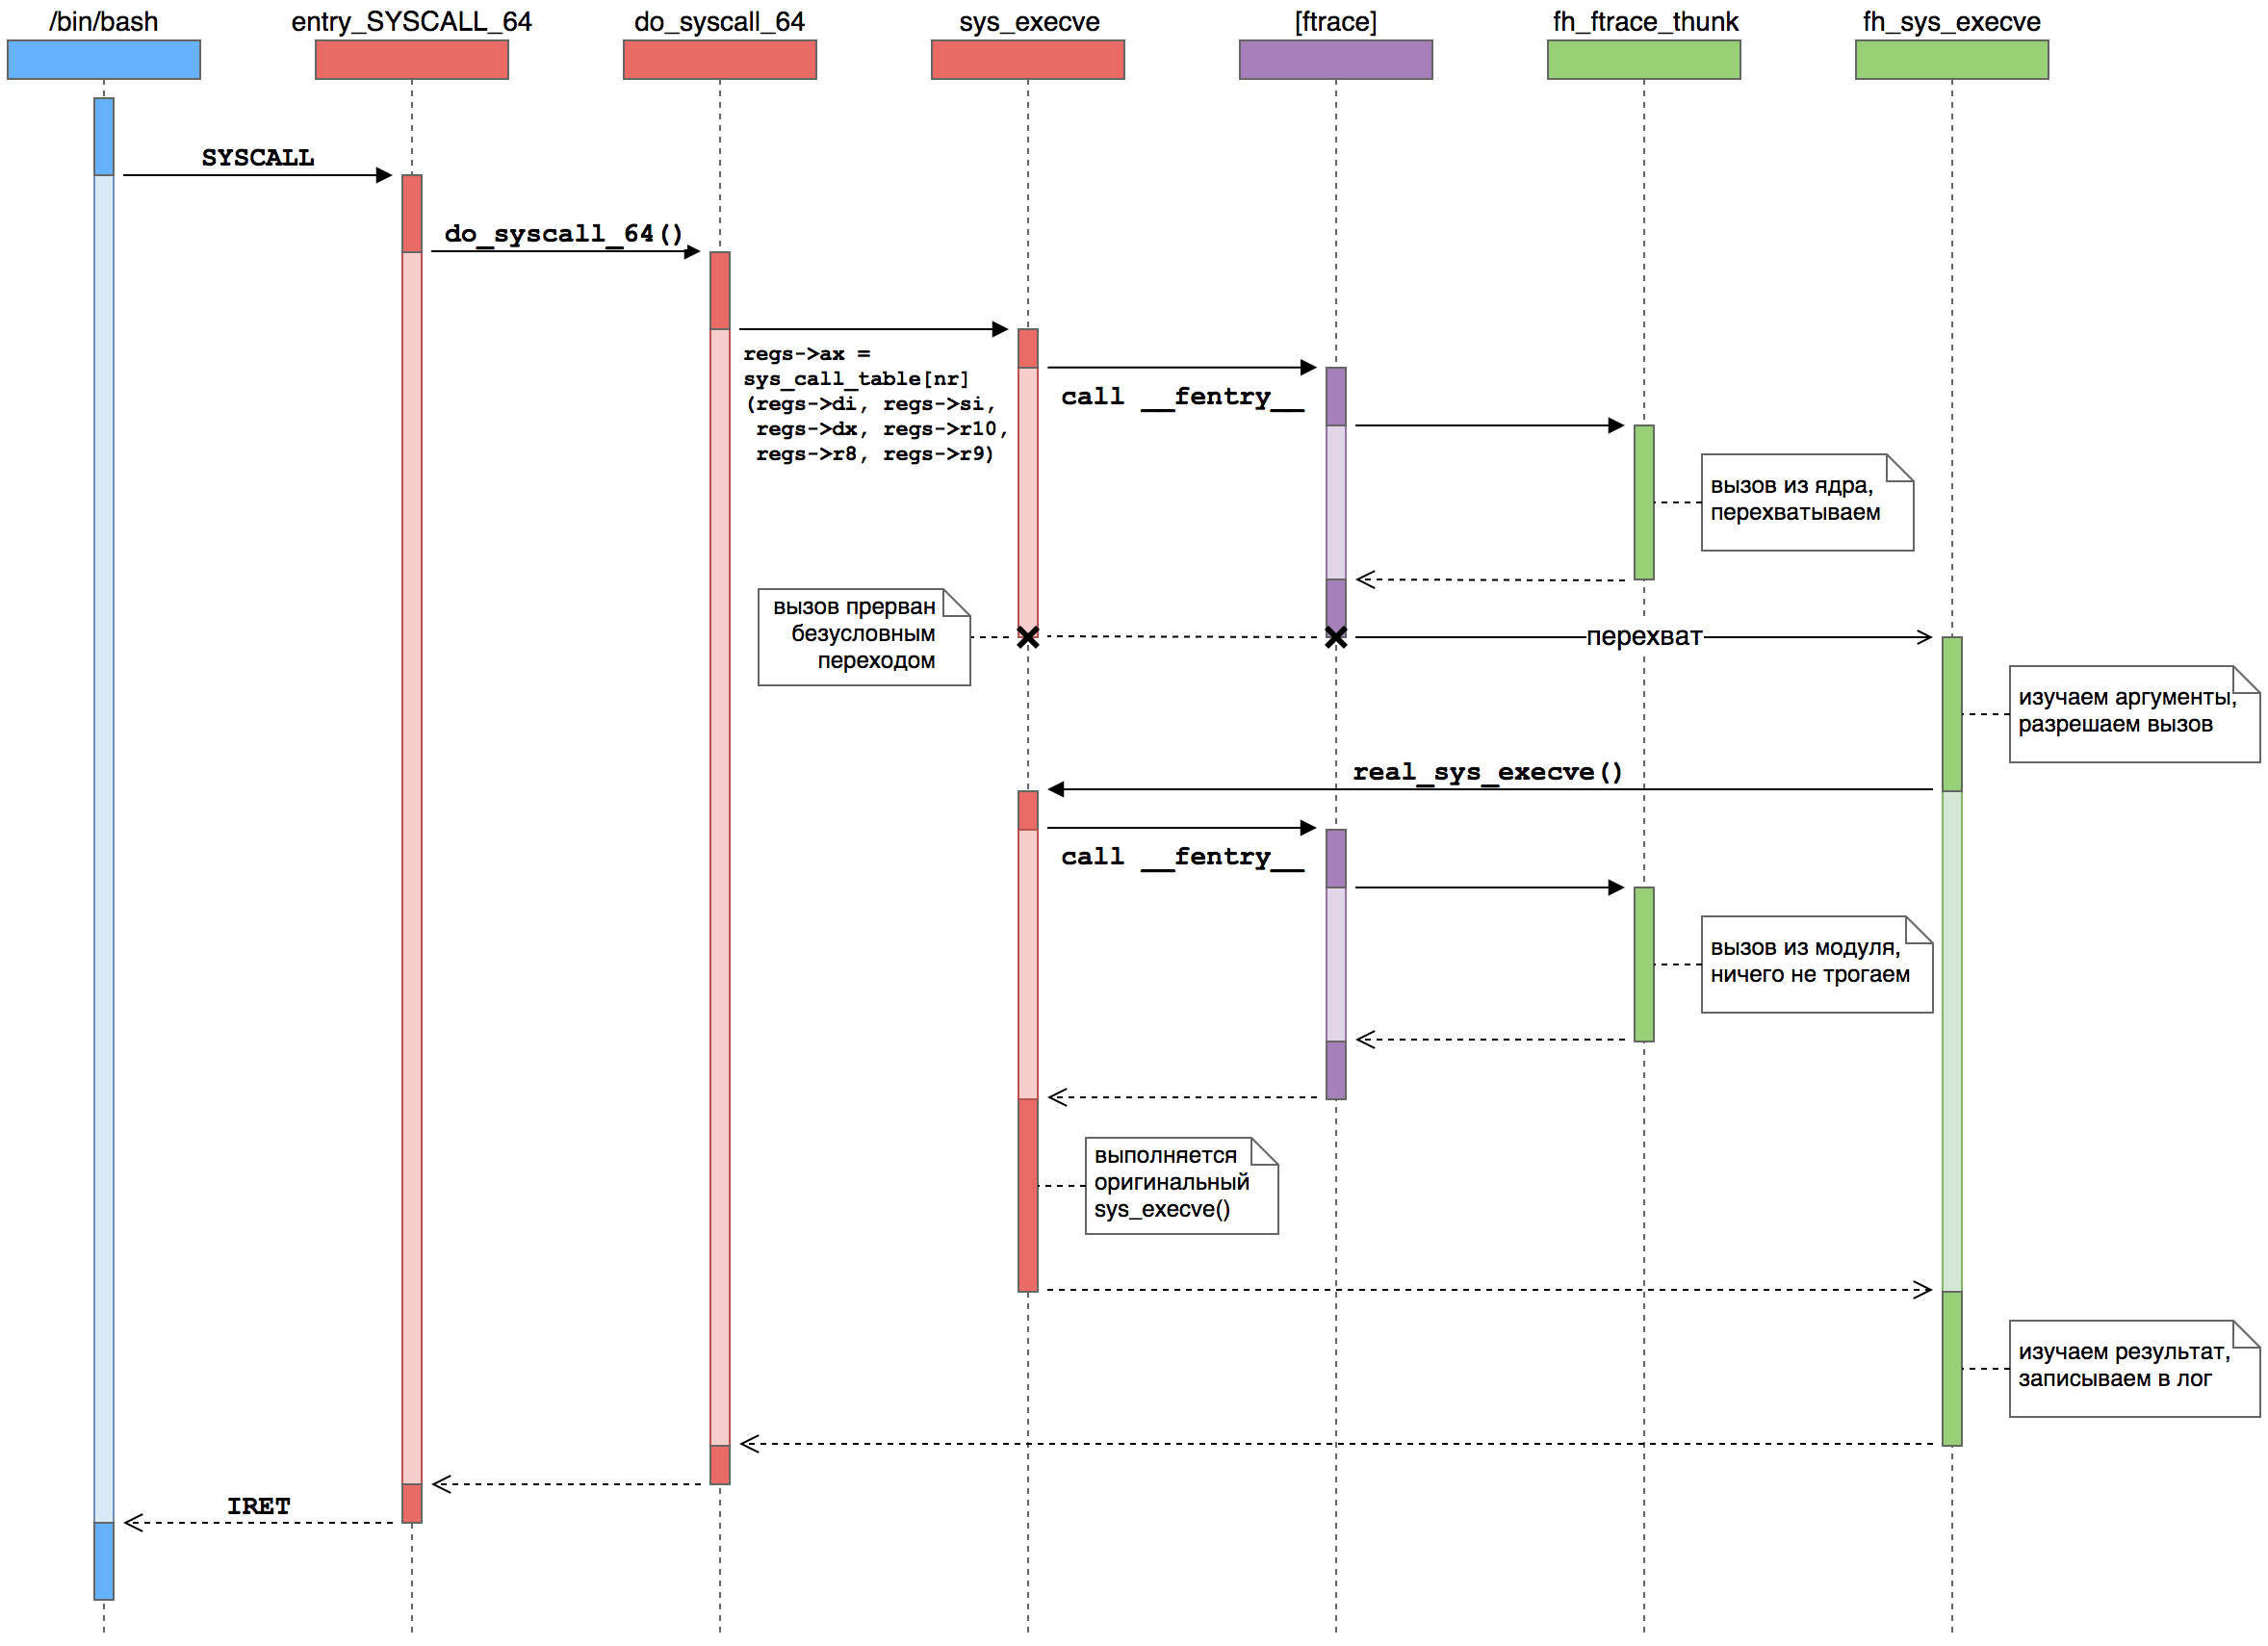
\includegraphics[width=1.0\textwidth]{img/hook_work_scheme.png}
	\caption{Алгоритм работы функции-перехватчика}
	\label{fig:spire00}
\end{figure}

\newpage
\section{Сервер}

Сервер описывается следующими структурами:
\begin{lstlisting}[language=c++,,escapeinside={(@}{@)},caption={tcp\_server\_service}]
// Структура, описывающая и хранящие данные о текущем соединении для каждого клиента
struct tcp_conn_handler_data {
	struct sockaddr_in *address;
	struct socket *accept_socket;
	int thread_id;
};

// Структура, описывающая и хранящие данные о текущих соединениях для всех клиентов
struct tcp_conn_handler {
	struct tcp_conn_handler_data *data[MAX_CONNS];
	struct task_struct *thread[MAX_CONNS];
	int tcp_conn_handler_stopped[MAX_CONNS];
};

// Структура, описывающая весь сервис
struct tcp_server_service {
	int running;
	struct socket *listen_socket;
	struct task_struct *thread;	
	struct task_struct *accept_thread;
};
\end{lstlisting}

\subsection{Алгоритм работы сервера}

При загрузке модуля, выделяется память под структуры tcp\_server\_service и tcp\_conn\_handler, running устанавливается в 1 и создается поток, слушающий, все приходящие соединения. Этому потоку передается на вход функция tcp\_server\_listen, которая делает стандартную последовательность действий для любого сервера, а именно: заполняет структуру sockaddr\_in, далее вызывает функции bind и listen. После создается новый поток для принятия соединений, ему на вход передается функция tcp\_server\_accept. Ранее созданный поток переходит в режим ожидания событий. 

Соединения на сервере работают по принципу keep-alive, это значит, что не рвется соединение с клиентом, а постоянно что-то записывается в сокет. Поэтому необходимо, чтобы клиенты не блокировали друг-друга. После того, как соединение принято функцией accept и заполнился сокет для каждого клиента, обработка соединения передается новому потоку, чтобы можно было принимать клиентов дальше.

Преимущества подхода:
\begin{itemize}
	\item Клиенты не блокируют и не ждут друг-друга
	\item Клиенты никак не взаимодействуют между собой
	\item Падение клиента не влияет на работу системы
\end{itemize}

Недостатки:
\begin{itemize}
	\item На каждого клиента создается новый поток, а значит будет создано N потоков в пространстве ядра на N клиентов. Это несомненно плохо, потому что больше задач будет бороться за получение кванта процессорного времени.
	\item Отправка данных клиенту происходит из функции перехватчика, поэтому требовуется каким-то образом передать ей данные о соединении. Самый простой способ - глобальный массив клиентов. В этом подходе есть существенная проблема: если описать несколько функций перехватчиков и передавать данные одним и тем же клиентам, то будет конкурентный доступ к этому массиву. В функциях перехватчиках нельзя вызывать блокировки, в связи с тем, что они могут повесить систему.
\end{itemize}

%%% Local Variables:

%%% mode: latex
%%% TeX-master: "rpz"
%%% End:
%--количество цветов
%||количество пикселей